\section{Issue tracking}

\begin{frame}{Issue tracking on GitLab Kanban boards} 
    \framesubtitle{Why use issue tracking?}
    \vfill

    Coordinating work on shared text-based information: different people editing same files.\\ 
    Tracking the status of tasks, bugs, and ideas in one place.\\
    Avoiding situations like these:
    \begin{itemize}  
        \item Why did we try that model a year ago?
        \item What was that bug in X?
        \item Meetings for discussing task status. 
            \begin{itemize}
                \item Fine for a Ph.D. student in a single project, not so fine for a postdoc with 5 projects. 
                \item Not necessary if no input is required, only the status update. 
            \end{itemize}
    \end{itemize}

\end{frame}

\begin{frame}{Issue tracking on GitLab Kanban boards} 
    \framesubtitle{Kanban board at TUGitLab}
    \vfill

    \begin{figure}
        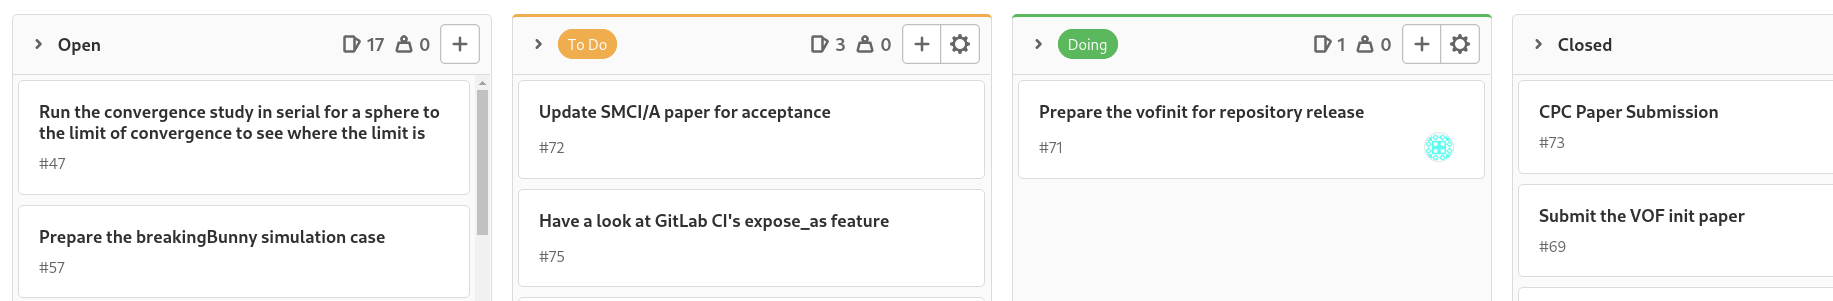
\includegraphics[width=\textwidth]{figures/kanban-board-gitlab.png}
    \end{figure}

    \begin{itemize}
        \item Create tasks and update their status.  
        \item Great for problems / bugs that can't be solved immediately. 
        \item Descriptions and comments can be done within the tasks (no searching through emails).  
    \end{itemize}

\end{frame}

\begin{frame}{Issue tracking on GitLab Kanban boards} 
    \framesubtitle{Progress Tracking Cards I}
    \vfill

    \href{}{Progress Tracking Cards}\footnote{\href{https://bssw.io/}{https://bssw.io/} Better Scientific Software} are great for teamwork.
    \begin{enumerate}  
        \item Title the task that will be solved by the team in terms of what will be achieved.
        \item Separate the task into subtasks and mention who is responsible for what. 
            \begin{itemize}
                \item Each sub-task is titled based on the achieved result.
            \end{itemize}
        \item Comment in the task, chat on Slack (Discord, ...) if more discussion is necessary, Zoom / meet if even more discussion is necessary.
    \end{enumerate}

\end{frame}
